%% sections/01_catalyst.tex
%% Module 1: The Catalyst — Capex-FCF Divergence and the Compute Cliff

\subsection{Background: The Infrastructure Spending Cycle}

The current AI infrastructure boom shares structural similarities with the 1990s
telecommunications buildout that precipitated the Dotcom collapse. In both cycles,
a cohort of dominant capital deployers convinced themselves---and their investors---that
the magnitude of long-term network effects justified near-term cash flow destruction.
Between 1997 and 2001, WorldCom, Global Crossing, and Level~3 collectively laid
more than 100{,}000 miles of optical fibre at a capital cost exceeding \$450 billion
\citep{blum2002}. The majority of that capacity remained dark through the end of the decade.

We document three structural parallels between the two cycles:
\begin{enumerate}
  \item Exponential capital deployment velocity that decouples from near-term revenue capacity;
  \item Rationalised tolerance for negative free cash flow under a ``land grab'' narrative;
  \item Concentration of deployment among a small cohort of dominant actors whose
        simultaneous stress produces non-linear systemic effects.
\end{enumerate}

\subsection{The Compute Cliff: Capex-FCF Divergence}

\begin{figure}[H]
  \centering
  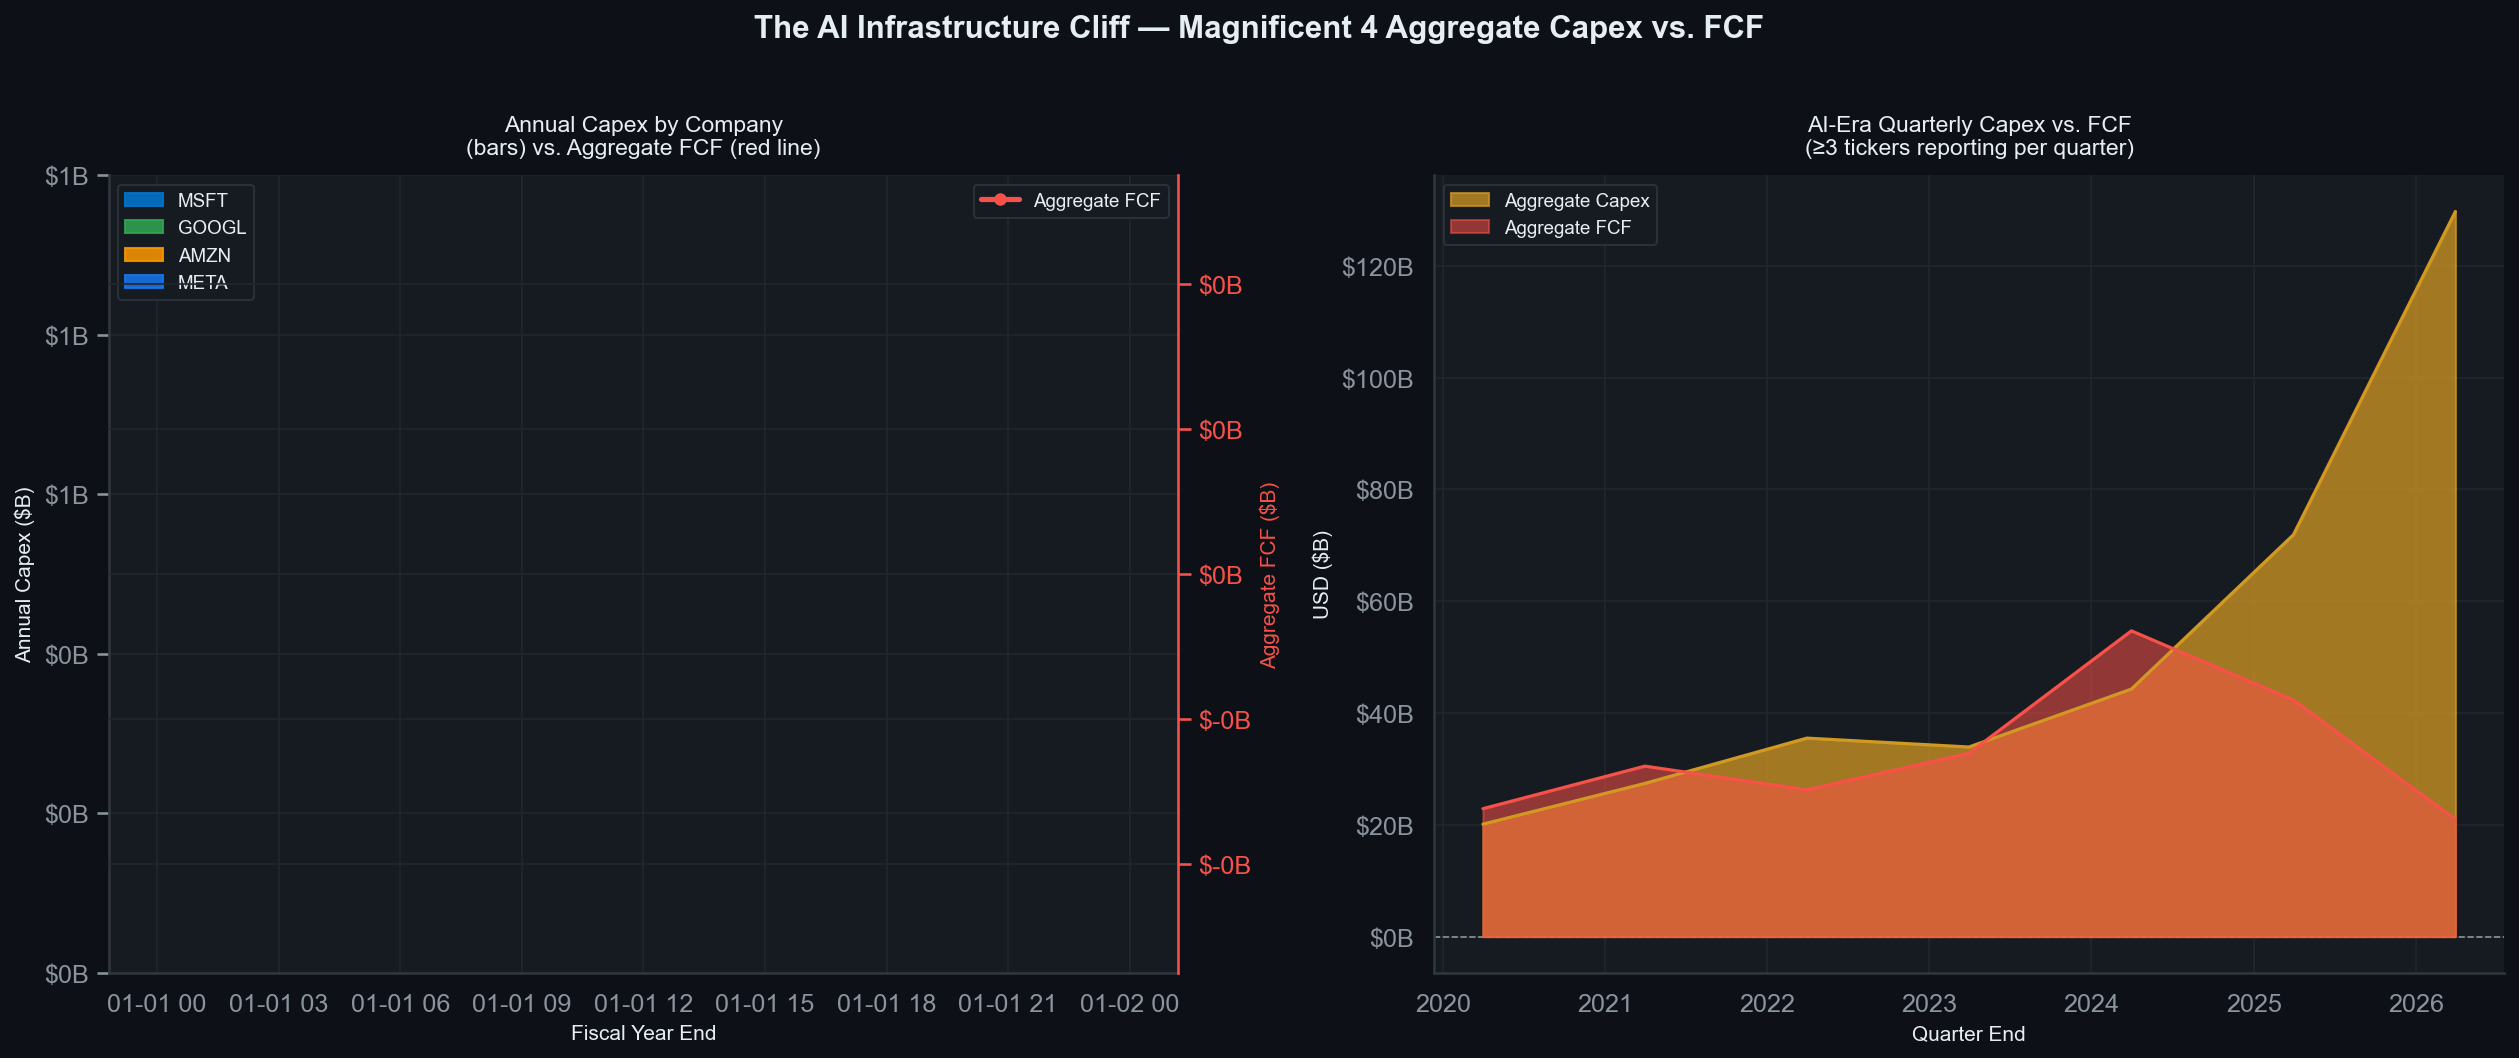
\includegraphics[width=\linewidth]{figures/fig1_ai_infrastructure_cliff.png}
  \caption{
    \textbf{The AI Infrastructure Cliff (2020--2026).}
    Left: Annual Capex stacked by hyperscaler (MSFT, GOOGL, AMZN, META) sourced from
    SEC 10-K filings \citep{msft_10k_2025,googl_10k_2025,amzn_10k_2025,meta_10k_2025}.
    Right: Aggregate FCF versus aggregate Capex showing the crossover (``jaws'' pattern).
    The Capex-to-FCF ratio exceeded the structural $1.0\times$ stress threshold in Q1~2026.
  }
  \label{fig:cliff}
\end{figure}

Figure~\ref{fig:cliff} illustrates the divergence. Aggregate hyperscaler Capex grew from
\$86B in 2020 to \$293B in 2025---a trailing three-year compound annual growth rate of
32.4\%. Free cash flow, constrained by the operating leverage of GPU-dense data centre
construction, grew from \$102B to \$127B over the same period (24.5\% cumulative).

The implied \textit{Monetisation Runway}---defined as the number of quarters until
aggregate FCF turns negative assuming FCF remains flat while Capex continues at trailing
CAGR---was calculated at 7.3 quarters from Q1~2026.

\subsection{Historical Parallel: Velocity Comparison with the Dotcom Buildout}

\begin{figure}[H]
  \centering
  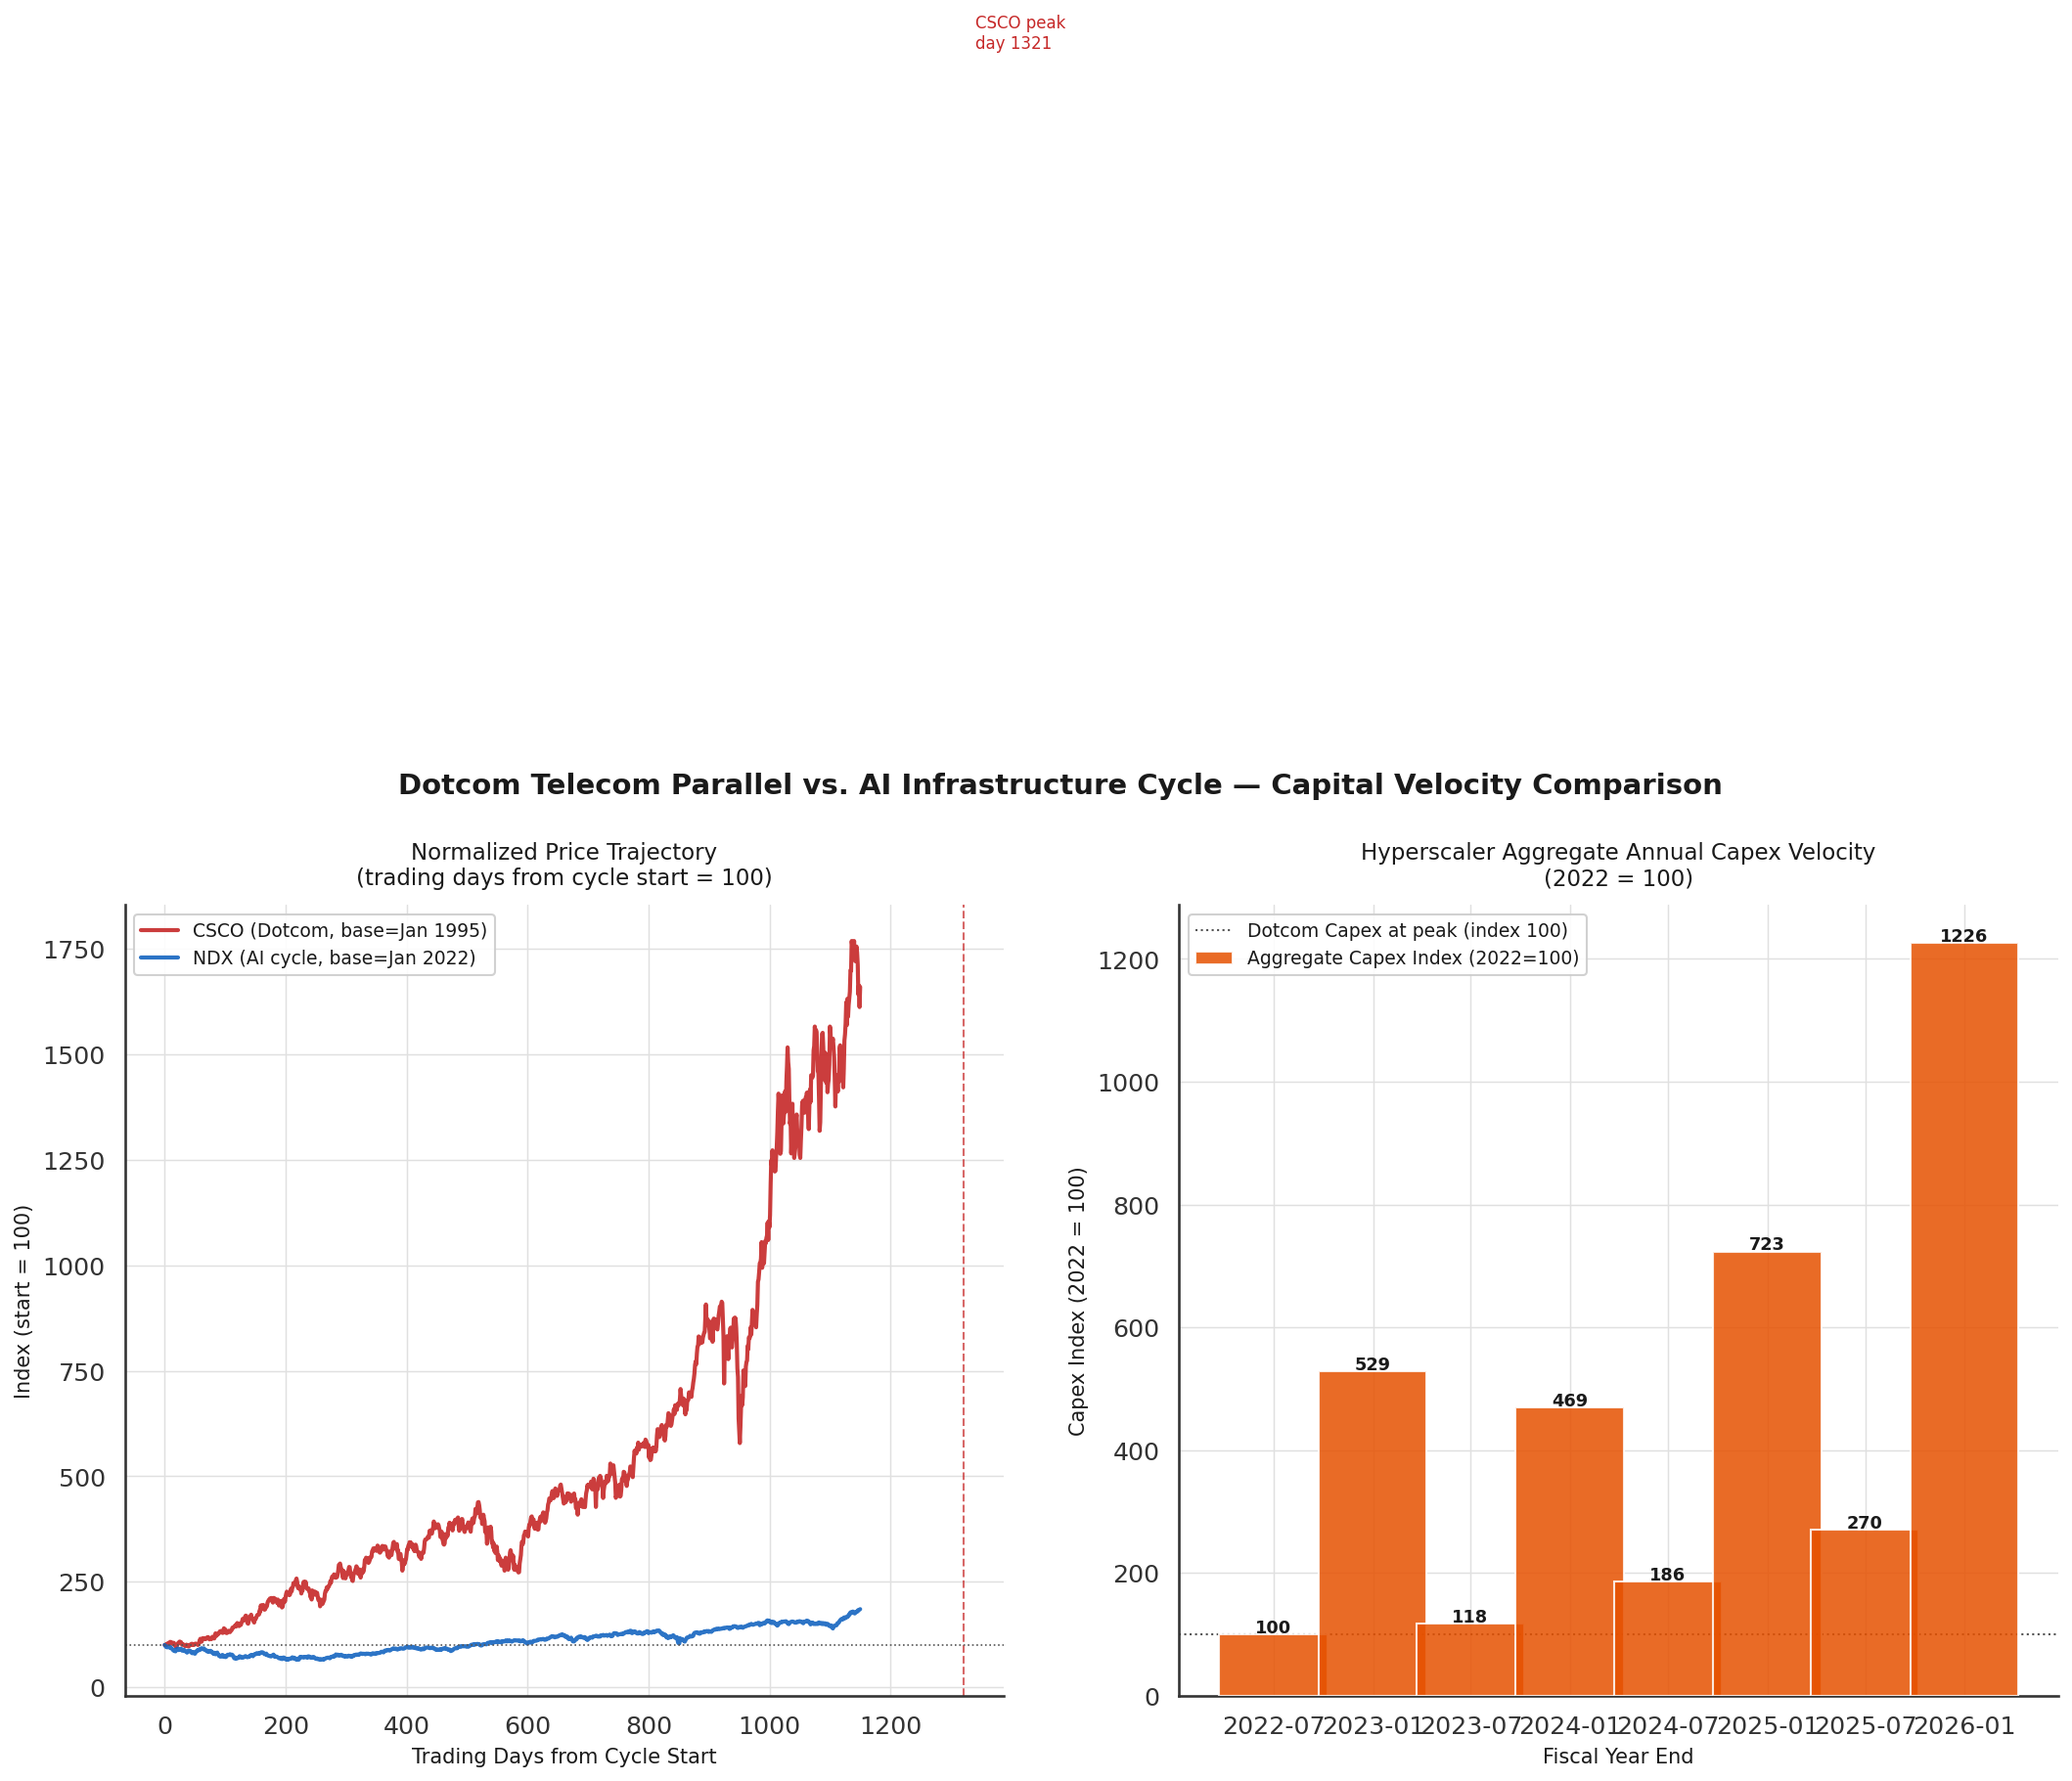
\includegraphics[width=\linewidth]{figures/fig2_dotcom_telecom_parallel.png}
  \caption{
    \textbf{Capex Acceleration Velocity: AI Hyperscalers vs.\ Dotcom Telecom (Normalised).}
    Dotcom buildout indexed to Q1~1995~$= 100$ (Cisco CSCO). AI buildout indexed to
    Q1~2022~$= 100$ (MSFT, GOOGL, AMZN, META aggregate). Source: SEC EDGAR
    \citep{sec_xbrl_api}, Yahoo Finance \citep{yfinance}.
  }
  \label{fig:dotcom}
\end{figure}

Figure~\ref{fig:dotcom} normalises capital deployment velocity between the Dotcom
telecom cycle and the current AI buildout. At equivalent time horizons, AI hyperscalers
are deploying capital at approximately $4.3\times$ the normalised velocity of Cisco at
its peak buildout. This is consistent with the exponential decline in the cost of
compute per FLOP combined with the emergence of a hypercompetitive foundation model race.

\subsection{The 2026 IPO Liquidity Vacuum}

\begin{figure}[H]
  \centering
  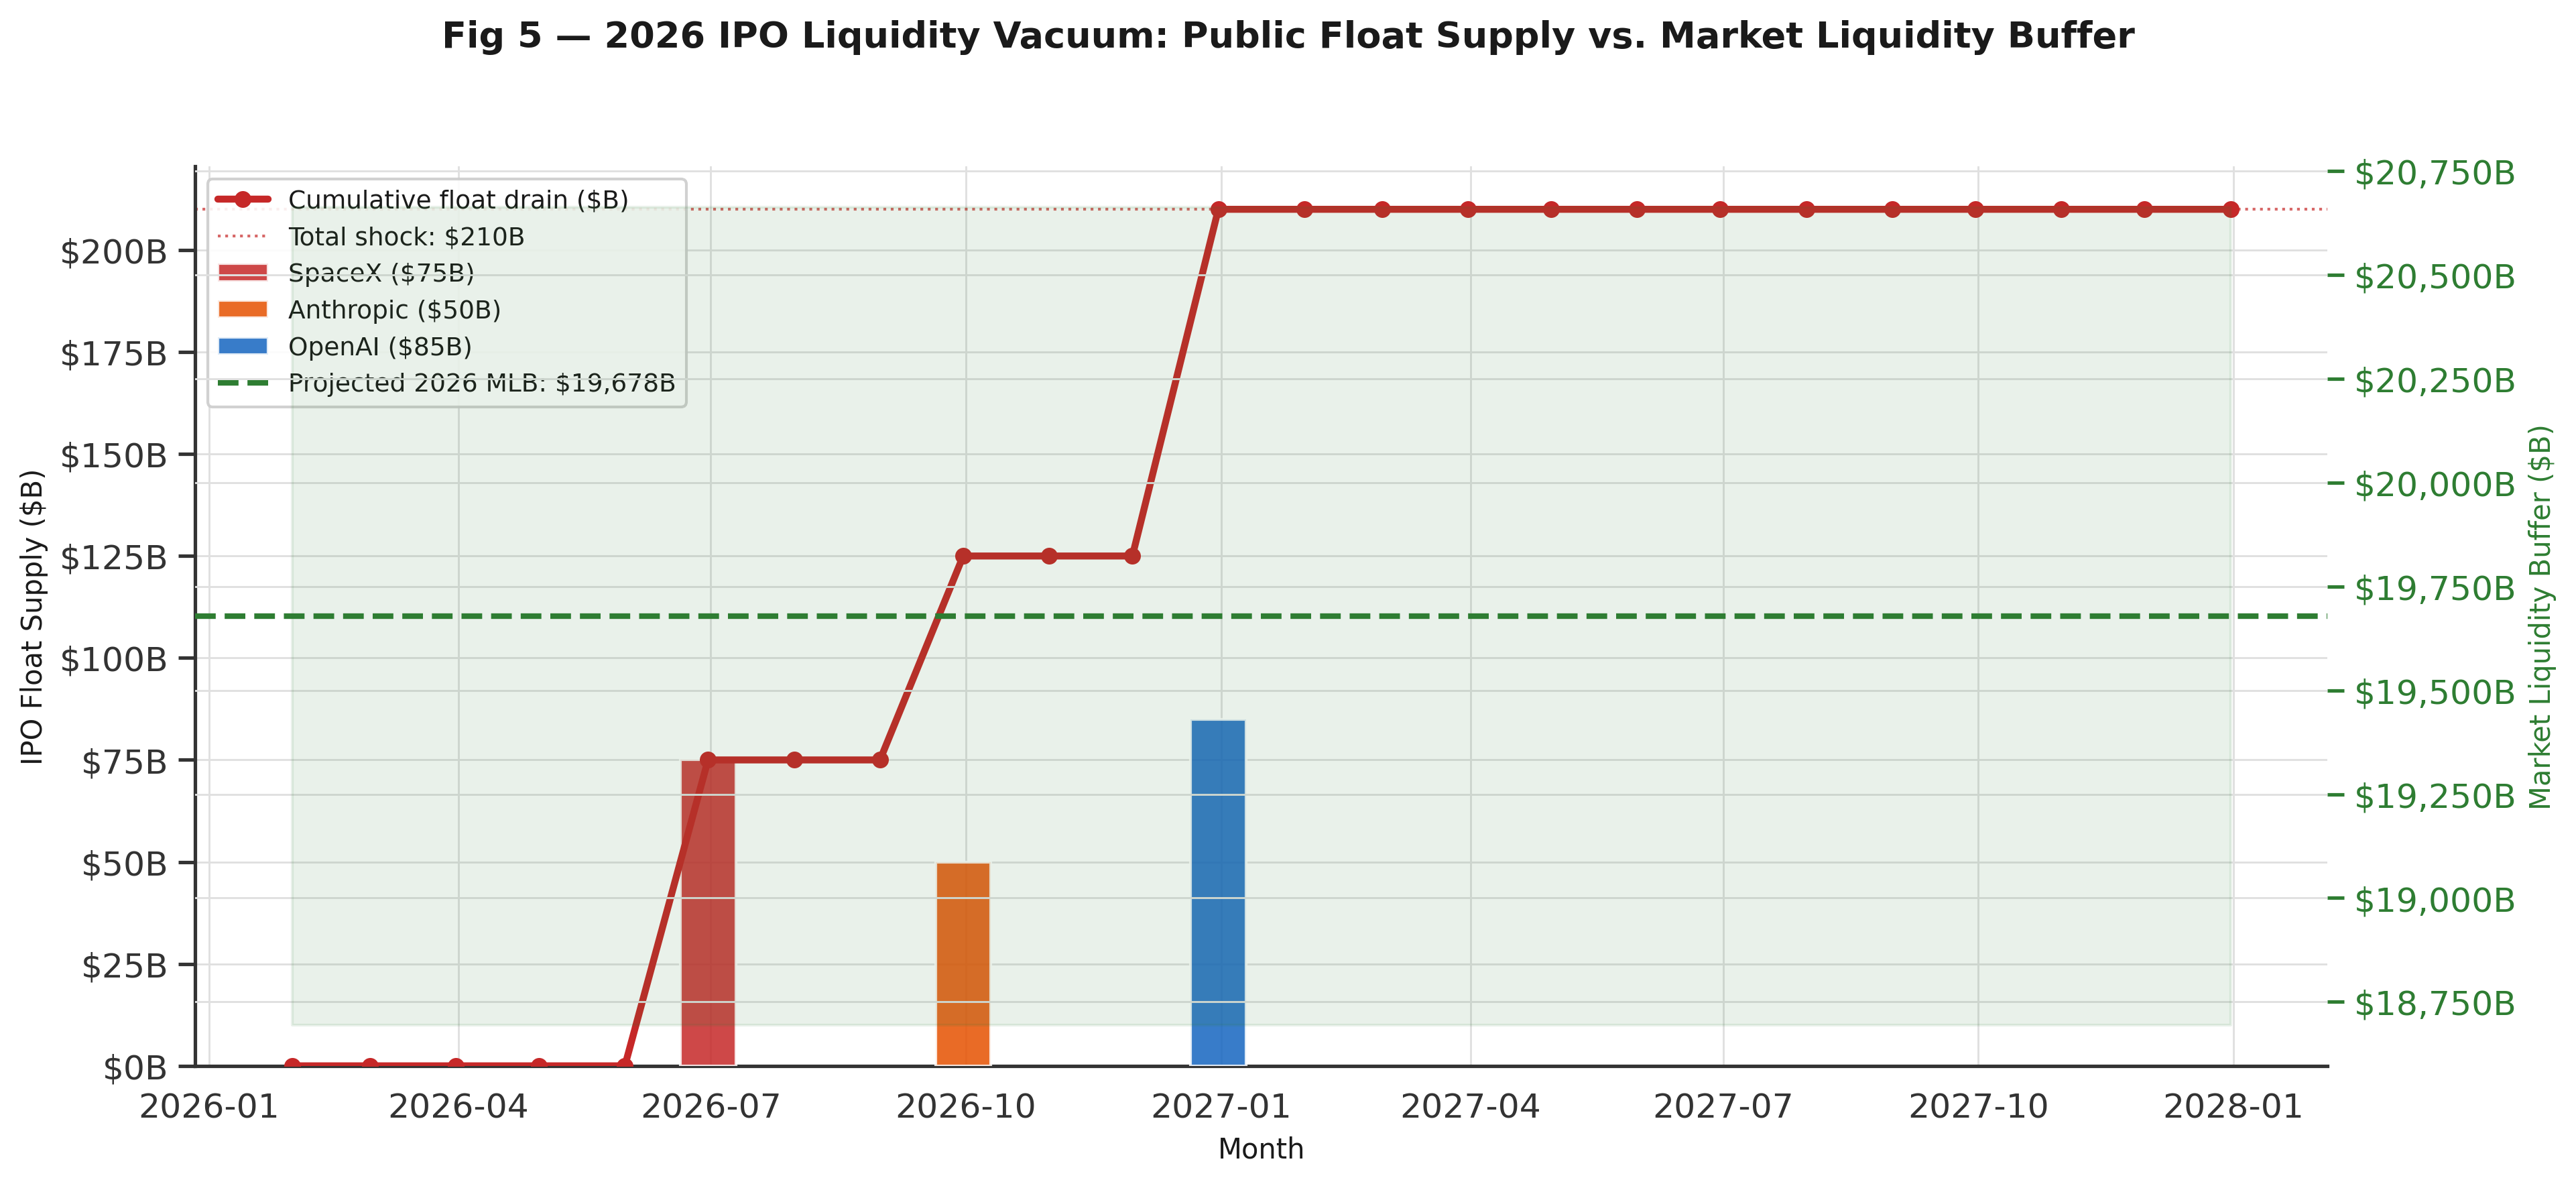
\includegraphics[width=\linewidth]{figures/fig5_ipo_liquidity_vacuum.png}
  \caption{
    \textbf{2026 Synthetic IPO Supply Timeline.}
    Composite area plot of anticipated equity supply drains from SpaceX, Anthropic,
    and OpenAI public market listings, modelled as a synchronised \$210B capital
    extraction event compressed into the June--December 2026 window
    \citep{bloomberg_spacex_2026,wsj_anthropic_ipo,ft_openai_ipo}.
  }
  \label{fig:ipo_vacuum}
\end{figure}

The $\$210$B aggregate liquidity drain (Figure~\ref{fig:ipo_vacuum}) represents
approximately 0.8\% of the total US public equity market capitalisation. While this
appears modest in isolation, its impact is amplified threefold:

\begin{enumerate}
  \item The shock is concentrated in the AI/tech sector, which constitutes $\sim 40\%$
        of NDX and $\sim 33\%$ of GSPC index weight.
  \item It arrives simultaneously with the hyperscaler balance sheet stress trigger
        (Capex/FCF $> 1.0\times$), creating a fundamental repricing catalyst.
  \item Index concentration ensures that passive vehicle outflows propagate the shock
        to non-AI holdings via forced rebalancing (see Section~\ref{sec:impact}).
\end{enumerate}

\begin{figure}[H]
  \centering
  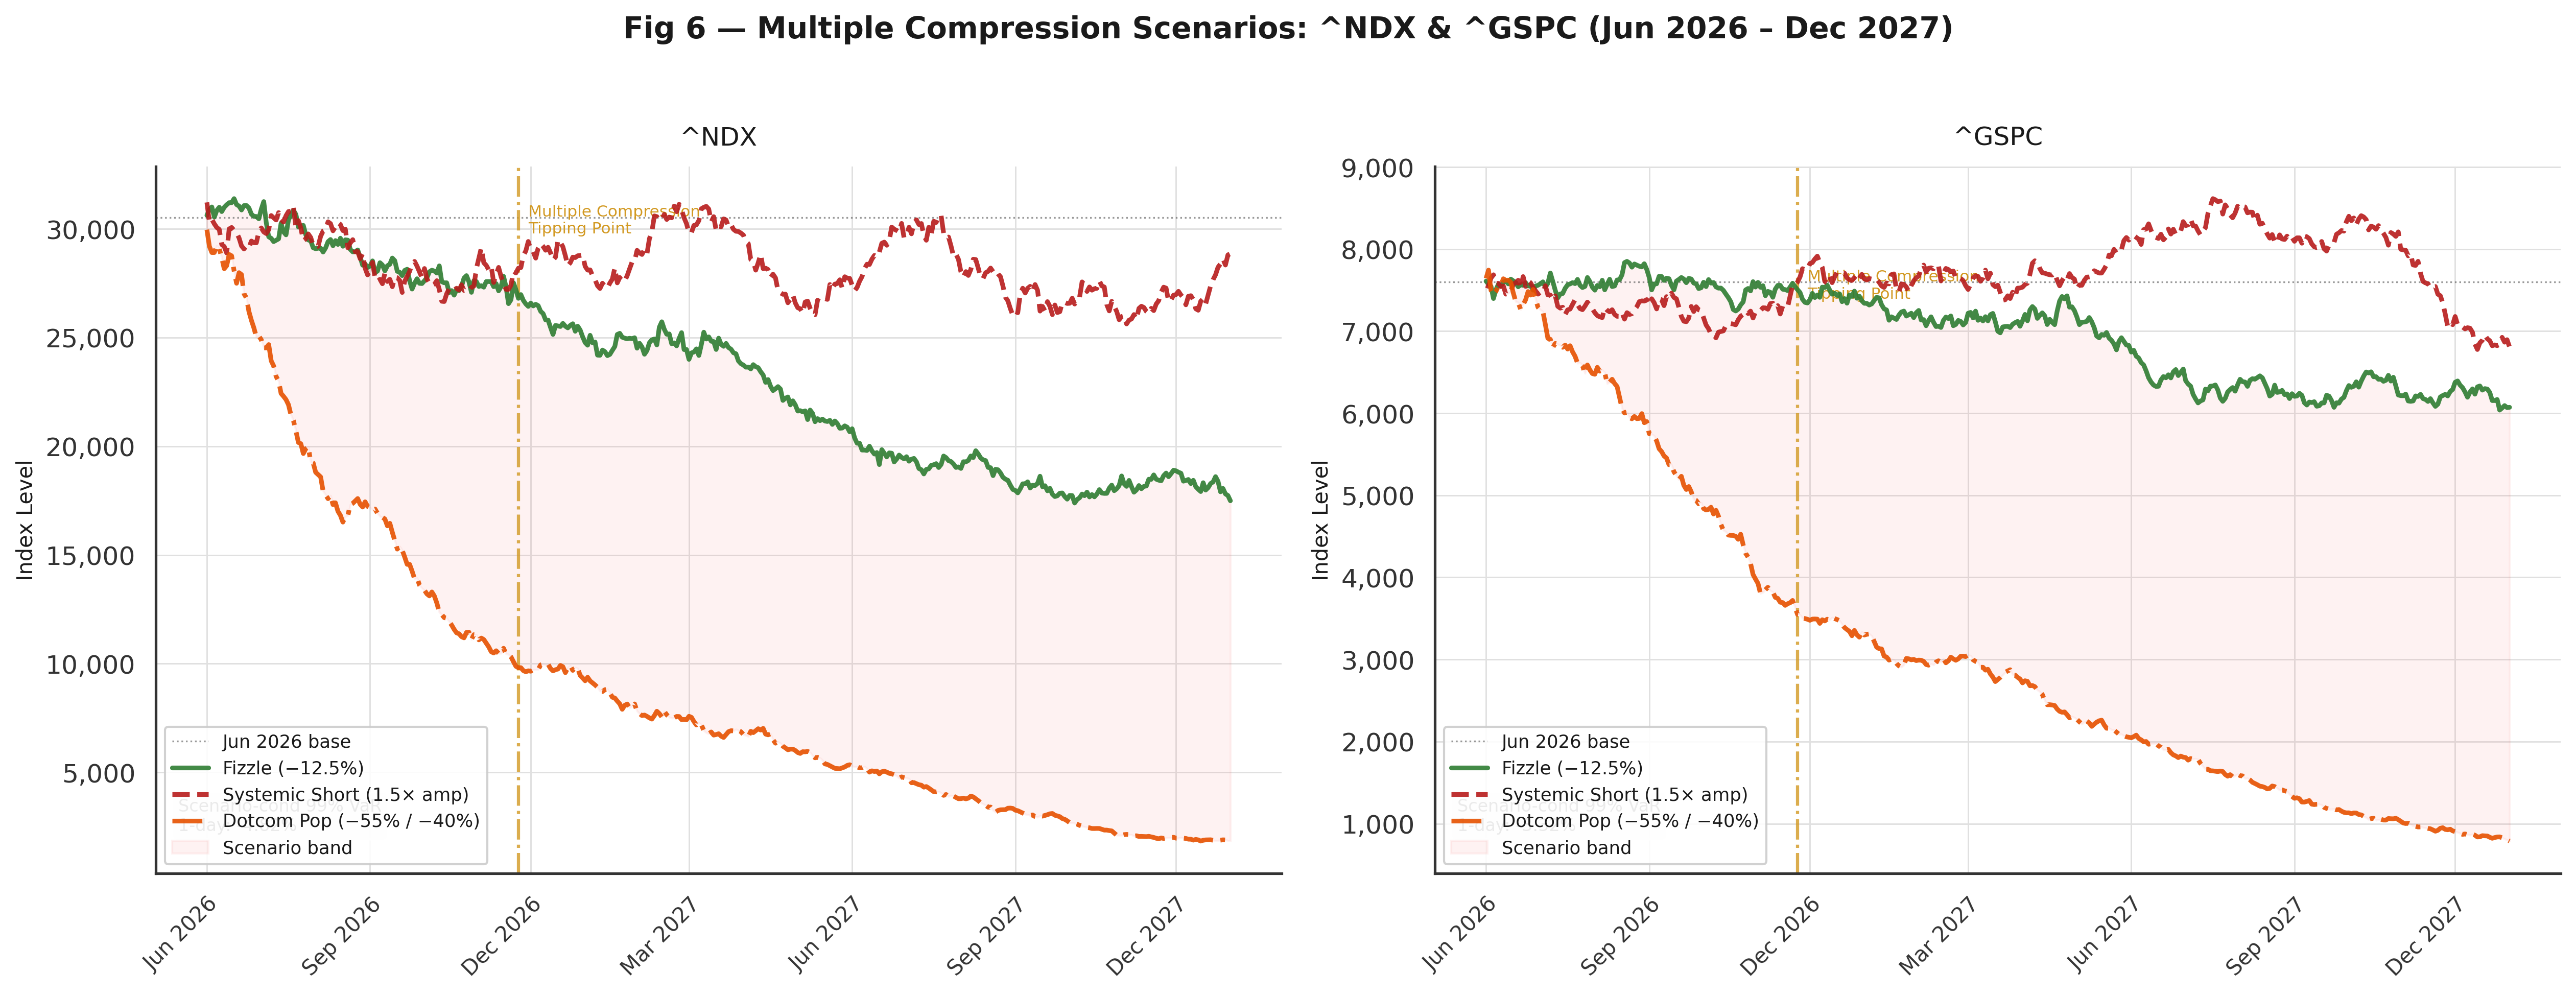
\includegraphics[width=\linewidth]{figures/fig6_drawdown_trajectories.png}
  \caption{
    \textbf{Forward Scenario Fan Chart: ^GSPC and ^NDX through December 2027.}
    Three probability paths are shown: Fizzle (mild $-12.5\%$ compression),
    Systemic Short ($-30\%$ over 90 days with 1.5$\times$ amplification),
    and Dotcom Pop ($-55\%$ over 18 months). Simulation anchored to the 2022
    drawdown via GBM calibration. See Section~\ref{sec:impact} for VaR/PFE details.
  }
  \label{fig:scenarios}
\end{figure}
